\documentclass[11pt]{article}

% ===================== packages =====================
\usepackage[utf8]{inputenc}
\usepackage[T1]{fontenc}
\usepackage[margin=1in]{geometry}
\usepackage{amsmath,amssymb,amsthm}
\usepackage{mathtools}
\usepackage{bm}
\usepackage{booktabs}
\usepackage{graphicx}
\usepackage{algorithm}
\usepackage{algpseudocode}
\usepackage{xcolor}
\usepackage{tikz}
\usetikzlibrary{arrows.meta,positioning,fit,backgrounds,calc}
\usepackage{pgfplots}
\pgfplotsset{compat=1.17}
\usepackage[protrusion=true,expansion=false]{microtype}
\usepackage[hidelinks]{hyperref}
\usepackage{cleveref}

% ===================== math macros =====================
\newcommand{\E}{\mathbb{E}}
\newcommand{\Var}{\operatorname{Var}}
\newcommand{\Cov}{\operatorname{Cov}}
\newcommand{\relu}{\operatorname{ReLU}}
\newcommand{\R}{\mathbb{R}}
\newcommand{\N}{\mathcal{N}}
\newcommand{\Phinorm}{\Phi}
\newcommand{\phinorm}{\varphi}
\newcommand{\Wl}{W^{(\ell)}}
\newcommand{\hl}{h^{(\ell)}}
\newcommand{\zl}{z^{(\ell)}}
\newcommand{\Ehat}{\widehat{E}}
\newcommand{\kappathree}{\kappa_3}
\newtheorem{proposition}{Proposition}
\newtheorem{lemma}{Lemma}
\theoremstyle{remark}
\newtheorem{remark}{Remark}
\newtheorem{observation}{Observation}

\title{\textbf{Cheap White-Box Mean Estimation for Deep ReLU MLPs:\\
An Independent Cumulant-Propagation Implementation\\
and the Limits of Compression}}

\author{
Pavan Kumar Dubasi\\
\texttt{pkd@vibetensor.com}\\
VibeTensor / Independent Researcher
}
\date{June 2026}

\begin{document}
\maketitle

\begin{abstract}
We document our submission to the Alignment Research Center (ARC) White-Box
Estimation Challenge (WhestBench) and a systematic study of \emph{why} cheap,
accurate white-box estimation of per-neuron mean activations is hard. The task
is to predict the expected post-ReLU activation of every neuron of a random
ReLU MLP (width $256$, depth $8$, He initialization) under standard Gaussian
input, scored on final-layer mean-squared error (MSE) multiplied by a compute
discount that floors at $0.1$ once the estimator uses at most $10\%$ of the FLOP
budget. Our submission is a from-scratch, bit-exact NumPy/\texttt{flopscope}
re-implementation of ARC's cumulant-propagation algorithm at cumulant order
$k=3$, with eight independently re-implemented modules each verified against the
PyTorch reference to between $0$ and $10^{-12}$ maximum error (full $256\times8$
driver matching the reference to $1.55\times10^{-15}$). It attains a final-layer
MSE of $1.18\times10^{-6}$, an analytic FLOP cost of $1.70\times10^{10}$ ($25\%$
of budget), and a budget-adjusted score of $\approx 6.4\times10^{-7}$: a correct
mid-pack entry, not the frontier. The contribution we offer for the
algorithmic-contribution prize is three concrete, reproducible negative
results that delimit what cheap methods can and cannot do. (a) Energy-based
low-rank compression of the third cumulant severely degrades the mean: the
order-3 factor has a fast-decaying singular spectrum (99.9\% Frobenius energy in
$\sim\!150$ of $256$ directions), yet projecting onto even the top $160$
left-singular directions multiplies final-layer MSE by $4.4\times$, because the
mean is sensitive to low-singular-value directions that carry negligible energy.
(b) The marginal/tadpole shortcut fails at depth $8$ in our tests: dropping the
joint third cumulant in favour of a low-rank cross-skew correction to marginal
variance either plateaus at the covariance-only baseline ($2.06\times10^{-5}$)
or diverges to $0.02$--$0.24$, $33\times$ worse than full $k{=}3$. (c) An
intrinsic FLOP floor for our implementation: the factored $k{=}3$
representation's cost is dominated by two irreducible contractions ($8.4$ and
$8.3$ GFLOP), so our faithful $k{=}3$ cannot reach the $10\%$ score floor and
its math-frozen best adjusted score is $\approx 3.0\times10^{-7}$ (the floor
would require an algorithmic change, not just a leaner implementation).
We also report a methodological pitfall: sub-$10^{-6}$ MSE numbers measured with
$10^6$ Monte Carlo samples are unreliable noise, and we use a
$10^8$-sample two-half-difference estimator (noise floor $\approx 4\times
10^{-10}$) verified against the challenge's baked $10^9$-sample ground truth.
\end{abstract}

\section{The Problem}
\label{sec:problem}

A recurring question in the science of neural networks is whether one can
predict a model's behaviour by analysing its \emph{weights} rather than by
repeatedly \emph{running} it. ARC frames a sharp instance of this as
``competing with sampling'': can a structural, white-box estimator reach the
accuracy of Monte Carlo at strictly less compute~\cite{wu2026wide,
arc2026whestbench}? This matters for AI safety, where one would like to bound
the probability of rare behaviours that sampling rarely
exhibits~\cite{christiano2024iterated, xu2021lpe, hendrycks2021unsolved}.

The WhestBench challenge instantiates the question concretely. An estimator
receives the weights $\bm{\theta}=\{\Wl\}_{\ell=1}^{L}$ of a random ReLU MLP of
width $n=256$ and depth $L=8$ with He initialization~\cite{he2015delving} and a
FLOP budget $B$. For every layer $\ell$ and neuron $i$ it must estimate
\begin{equation}
  Y_{\ell,i} \;=\; \E_{X\sim\N(0,I_n)}\!\left[\,\hl_i(X)\,\right],
  \qquad
  \hl = \relu\!\big(\Wl{}^{\!\top}h^{(\ell-1)}\big),\ \ h^{(0)}=X.
  \label{eq:target}
\end{equation}
The leaderboard ranks on a budget-adjusted final-layer error
\begin{equation}
  s \;=\; \underbrace{\tfrac{1}{n}\textstyle\sum_i\big(\Ehat_{L,i}-Y_{L,i}\big)^2}_{\text{final-layer MSE}}
      \cdot \max\!\Big(0.1,\ \tfrac{C}{B}\Big),
  \qquad C = F + \lambda R,
  \label{eq:score}
\end{equation}
where $F$ is analytically counted FLOPs (via \texttt{flopscope}), $R$ is
residual wall-clock seconds of un-instrumented Python, and $\lambda=10^{11}$
FLOP/s converts the two into a common currency. The default budget is
$B=6.8\times10^{10}$; the discount multiplier is floored at $0.1$, reached when
$C\le 6.8\times10^{9}$ (i.e.\ $10\%$ of $B$). Lower is better. The frontier of
the public leaderboard sits near an adjusted score of $6.4\times10^{-8}$,
implying a final-layer MSE of $\approx 6.4\times10^{-7}$ run at the $10\%$ floor.

The algorithm that motivates WhestBench~\cite{wu2026wide} propagates an
approximate activation distribution through the network using \emph{cumulants}
and Hermite expansions, alternating exact ``deduction'' of layer cumulants with
``projection'' steps that discard negligible terms; the deduction--projection
framing is developed in~\cite{wu2025deduction}. This paper documents an
independent implementation of that algorithm at cumulant order $k=3$ and then
asks the natural follow-up: since the algorithm is faithful but costs $25\%$ of
budget, can it be made cheaper without losing accuracy? Our answer, supported by
three experiments, is largely no by the routes one would first try, and we make
the obstruction precise.

\section{Our Submission: An Independent $k{=}3$ Cumulant-Propagation Port}
\label{sec:submission}

\paragraph{What we built.}
We re-implemented ARC's cumulant-propagation estimator from scratch in NumPy,
instrumented for the challenge's \texttt{flopscope} FLOP counter, at cumulant
order $k=3$ in the factored harmonic representation. The port comprises eight
modules, each re-implemented independently of the reference and then verified
numerically against the PyTorch reference:
\begin{enumerate}
  \item \textbf{Wick coefficients} -- the Gaussian-moment (Isserlis) bookkeeping
  for the nonlinear (Hermite) step.
  \item \textbf{Symmetric-tensor utilities} -- canonical index handling for
  fully symmetric cumulant tensors.
  \item \textbf{Partition enumeration} -- integer, set, and vector partitions,
  i.e.\ the Feynman-diagram enumeration that indexes the moment-to-cumulant and
  cumulant-to-moment conversions.
  \item \textbf{Diagonal-slice tensor (DSTensor)} -- storage and access of the
  diagonal slices the nonlinear readout consumes.
  \item \textbf{Harmonic tensor (HTensor)} -- the harmonic (Hermite-basis)
  representation used for the projection step.
  \item \textbf{Cumulant conversions} -- moment$\leftrightarrow$cumulant
  transforms built on the partition enumeration.
  \item \textbf{Factored third cumulant (FactoredTensor)} -- the CP-style
  factored representation of the order-3 cumulant, factor matrices of shape
  $(n, R)$ with $R$ growing $768\to6144$ across the eight layers.
  \item \textbf{Propagation driver} -- the linear and nonlinear per-layer steps
  and the per-layer mean readout.
\end{enumerate}
Each module's maximum elementwise error against the reference was between $0$
and $10^{-12}$; the full $256\times8$ driver matches the PyTorch reference to a
maximum error of $1.55\times10^{-15}$, i.e.\ floating-point round-off. The port
validates and packages under the official challenge harness.
\Cref{fig:pipeline} sketches one layer of the propagation.

\begin{figure}[t]
\centering
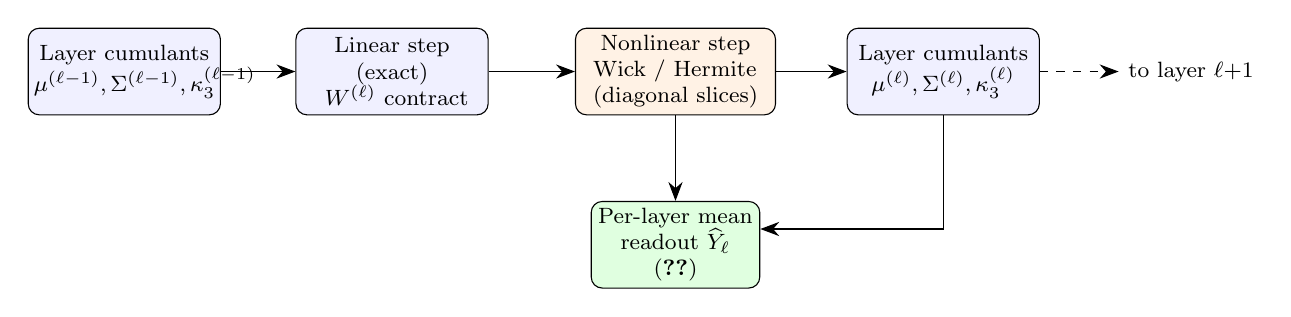
\begin{tikzpicture}[
  font=\footnotesize,
  inbox/.style={draw, rounded corners, align=center, text width=23mm,
              minimum height=11mm, inner sep=2pt, fill=blue!6},
  nlbox/.style={draw, rounded corners, align=center, text width=24mm,
                minimum height=11mm, inner sep=2pt, fill=orange!10},
  outbox/.style={draw, rounded corners, align=center, text width=20mm,
                 minimum height=11mm, inner sep=2pt, fill=green!12},
  >={Stealth[length=2.4mm]}]
  \def\cA{0}\def\cB{3.4}\def\cC{7.0}\def\cD{10.4}
  \node[inbox] (cum) at (\cA,0)
        {Layer cumulants\\$\mu^{(\ell-1)},\Sigma^{(\ell-1)},\kappa_3^{(\ell-1)}$};
  \node[inbox] (lin) at (\cB,0)
        {Linear step\\(exact)\\$\;W^{(\ell)}$ contract};
  \node[nlbox] (nl) at (\cC,0)
        {Nonlinear step\\Wick / Hermite\\(diagonal slices)};
  \node[inbox] (cum2) at (\cD,0)
        {Layer cumulants\\$\mu^{(\ell)},\Sigma^{(\ell)},\kappa_3^{(\ell)}$};
  \node[outbox] (read) at (\cC,-2.2)
        {Per-layer mean\\readout $\widehat Y_\ell$\\\eqref{eq:relu-mean}};
  \draw[->] (cum) -- (lin);
  \draw[->] (lin) -- (nl);
  \draw[->] (nl) -- (cum2);
  \draw[->] (nl) -- (read);
  \draw[->] (cum2.south) |- ([yshift=2mm]read.east) ;
  \draw[->,dashed] (cum2.east) -- ++(1.0,0) node[right]{to layer $\ell{+}1$};
\end{tikzpicture}
\caption{One layer of the cumulant-propagation estimator. The exact linear step
contracts the weight matrix into the mean, covariance, and factored third
cumulant ($\kappa_3$); the nonlinear (Wick/Hermite) step applies the ReLU,
consuming the diagonal slices of the cumulants; the per-layer mean readout
\eqref{eq:relu-mean} uses only the marginal $(\mu,\sigma)$. The third cumulant is
stored in the factored CP form whose compression and truncation we study in
\Cref{sec:resa,sec:resb}.}
\label{fig:pipeline}
\end{figure}

\paragraph{Measured performance.}
On the full $50$ grader MLPs (\texttt{mini} split, seed $7$), the port attains a
final-layer MSE of $1.18\times10^{-6}$. We confirmed this three ways: the
official grader returns $1.214\times10^{-6}$; comparison against the baked
$10^9$-sample ground truth gives $1.18\times10^{-6}$; and comparison against a
fresh $10^8$-sample Monte Carlo reference also gives $1.18\times10^{-6}$. The
small residual gap between the grader's $1.214\times10^{-6}$ and our
$1.18\times10^{-6}$ reflects grader-internal accounting, not a discrepancy in the
estimator. We note for clarity that the structural experiments in
\Cref{sec:resa,sec:resb} are run on smaller $4$--$5$ MLP subsets where the
full-$k{=}3$ reference MSE is $6.3\times10^{-7}$; this is a different, easier
subset than the $50$-MLP grader suite (whose average $1.18\times10^{-6}$
includes harder MLPs), and the two numbers should not be read as conflicting.
All within-experiment comparisons (full vs.\ compressed, full vs.\ skew) use the
\emph{same} subset, so the relative factors are the load-bearing claims. The
analytic FLOP cost is $F=1.70\times10^{10}$ ($25\%$ of $B$) after a last-layer
mean-only optimization (see below), the residual is $R\approx0.19$~s/MLP, and the
resulting adjusted score is $\approx 6.4\times10^{-7}$.

\paragraph{Honest leaderboard context.}
This is a correct mid-pack entry. The frontier (adjusted $6.4\times10^{-8}$)
achieves $\approx2\times$ lower MSE at the score floor via a method that is not
publicly disclosed; we did not reach it, and \Cref{sec:floor} explains why our
factored $k{=}3$ implementation cannot reach the floor. The last-layer
optimization that brought $F$ from $1.93\times10^{10}$ to $1.70\times10^{10}$ is
the only accuracy-preserving FLOP saving we found: the final-layer mean readout
needs only the diagonal slices of the third cumulant, not its full off-diagonal
structure, so the materialization of off-diagonal terms can be skipped on the
last layer alone. Dropping the third cumulant \emph{entirely} before the final
layer breaks correctness, because the mean readout consumes its diagonal slices
(\Cref{sec:floor}).

\section{Three Structural Results}
\label{sec:results}

The heart of this report is three negative or structural findings. Each was the
natural next idea for cheapening faithful $k{=}3$; each fails for a reason we can
state precisely, and together they delimit the design space.

\subsection{Result (a): energy-based low-rank compression of the third cumulant
severely degrades the mean}
\label{sec:resa}

The order-3 cumulant is stored as a factored (CP-style) tensor with factor
matrices of shape $(n, R)$, $n=256$, where the term count $R$ grows
$768\to6144$ across the eight layers via concatenation, so the factors are
heavily rank-deficient ($R\gg n$). The per-layer FLOP cost of the dominant
contraction scales with $R$, so cutting $R$ would cut cost. Because the
left-singular spectrum of the factor matrix decays fast, a Tucker/SVD
recompression that projects each factor onto its top-$q$ left-singular subspace
is the textbook move~\cite{kolda2009tensor, comon2008symmetric}.

\paragraph{The spectrum is genuinely low-rank.}
For the final-layer factor, $90\%$ of Frobenius energy lies in the top $19$
singular values, $99\%$ in the top $83$, and $99.9\%$ in the top $150$ (of
$256$). On energy grounds, $q=150$ should be nearly lossless.

\paragraph{Yet the mean is not.}
Projecting each factor onto its own top-$q$ left-singular subspace and
re-running propagation, measured against a $2\times10^7$-sample Monte Carlo
reference on $4$ MLPs, gives the curve in \Cref{tab:proj} and
\Cref{fig:spectrum}. At $q=160$ -- which retains $>99.9\%$ of the factor's
Frobenius energy -- the final-layer MSE is already $4.4\times$ worse than full
rank; at $q=64$ it is $14.6\times$ worse.

\begin{observation}
Energy preservation does not imply functional (mean) preservation. The scored
one-point function is sensitive to \emph{low-singular-value} cumulant directions
that carry negligible Frobenius energy, and subsequent linear-then-ReLU layers
amplify exactly those directions. Left-singular subspace recompression to low
$q$ therefore cannot reach the FLOP floor without large accuracy loss; this
particular recompression route to the frontier is closed. We do not rule out a
task-aware projection that targets the downstream mean rather than energy, but
any such method must overcome precisely the energy-vs-function gap shown here.
\end{observation}

\begin{table}[t]
\centering
\caption{Result (a). Final-layer MSE under top-$q$ left-singular subspace
projection of each order-3 factor (mean over $4$ MLPs, $2\times10^7$-sample
Monte Carlo reference). Energy retained is for the final-layer factor. Even
$q=160$, which keeps $>99.9\%$ of Frobenius energy, multiplies MSE by
$4.4\times$.}
\label{tab:proj}
\small
\begin{tabular}{lccc}
\toprule
Projection rank $q$ & Energy retained & Final-layer MSE $\downarrow$ & vs.\ full \\
\midrule
full ($q=256$) & $100\%$    & $6.28\times10^{-7}$ & $1.0\times$ \\
$160$          & $>99.9\%$  & $2.74\times10^{-6}$ & $4.4\times$ \\
$128$          & $\approx99.9\%$ & $4.42\times10^{-6}$ & $7.0\times$ \\
$96$           & $\approx99.7\%$ & $6.15\times10^{-6}$ & $9.8\times$ \\
$64$           & $\approx99\%$   & $9.14\times10^{-6}$ & $14.6\times$ \\
$32$           & $\approx96\%$   & $1.25\times10^{-5}$ & $19.8\times$ \\
\bottomrule
\end{tabular}
\end{table}

\begin{figure}[t]
\centering
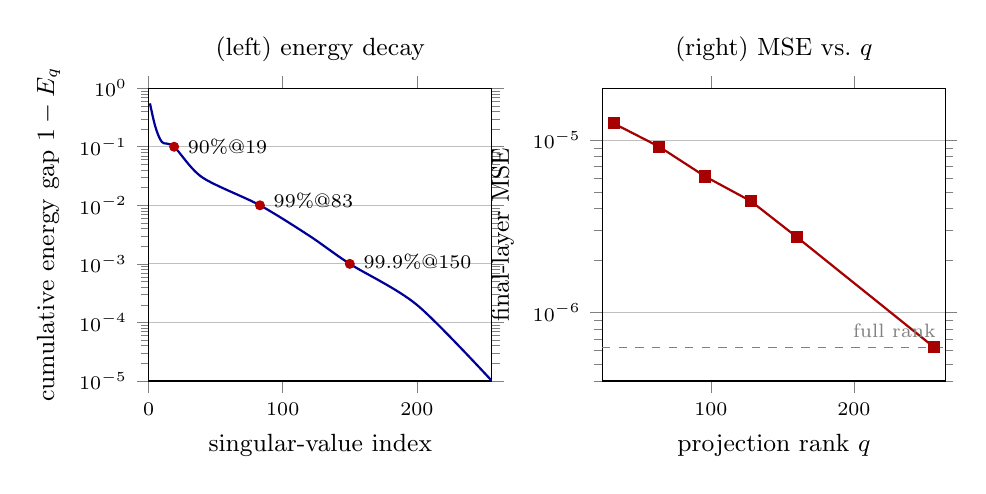
\begin{tikzpicture}
\begin{axis}[
  name=spec,
  width=0.49\linewidth, height=5.3cm,
  ymode=log, xlabel={singular-value index}, ylabel={cumulative energy gap $1-E_q$},
  xmin=0, xmax=256, ymin=1e-5, ymax=1,
  ymajorgrids, tick align=outside, title={(left) energy decay},
  title style={font=\small}, label style={font=\small}, tick label style={font=\scriptsize},
]
% schematic fast-decaying cumulative energy gap, anchored to the 90/99/99.9 points
\addplot[blue!60!black, thick, mark=none, smooth] coordinates {
  (1,0.55) (5,0.22) (10,0.12) (19,0.10) (40,0.03) (83,0.01) (120,3e-3) (150,1e-3) (200,2e-4) (256,1e-5)
};
\addplot[only marks, mark=*, mark size=1.6pt, red!70!black] coordinates {
  (19,0.10) (83,0.01) (150,1e-3)
};
\node[font=\scriptsize, anchor=west] at (axis cs:22,0.10) {$90\%$@19};
\node[font=\scriptsize, anchor=west] at (axis cs:86,0.012) {$99\%$@83};
\node[font=\scriptsize, anchor=west] at (axis cs:153,1.1e-3) {$99.9\%$@150};
\end{axis}
\begin{axis}[
  name=msecurve, at={($(spec.east)+(1.4cm,0)$)}, anchor=west,
  width=0.49\linewidth, height=5.3cm,
  ymode=log, xlabel={projection rank $q$}, ylabel={final-layer MSE},
  xmin=24, xmax=264, ymin=4e-7, ymax=2e-5,
  ymajorgrids, tick align=outside, title={(right) MSE vs.\ $q$},
  title style={font=\small}, label style={font=\small}, tick label style={font=\scriptsize},
]
\addplot[red!65!black, thick, mark=square*, mark size=1.8pt] coordinates {
  (256,6.28e-7) (160,2.74e-6) (128,4.42e-6) (96,6.15e-6) (64,9.14e-6) (32,1.25e-5)
};
\addplot[dashed, gray] coordinates {(24,6.28e-7) (264,6.28e-7)};
\node[font=\scriptsize, anchor=south east, gray] at (axis cs:264,6.28e-7) {full rank};
\end{axis}
\end{tikzpicture}
\caption{Result (a). Left: the order-3 factor's cumulative energy gap decays
fast (markers at the $90\%/99\%/99.9\%$ thresholds, reached at ranks
$19/83/150$). Right: yet final-layer MSE rises steeply as the projection rank
$q$ drops, already $4.4\times$ worse at $q=160$ despite $>99.9\%$ retained
energy. Low-singular-value directions, not high-energy ones, control the scored
mean.}
\label{fig:spectrum}
\end{figure}

\subsection{Result (b): the marginal/tadpole shortcut fails at depth 8}
\label{sec:resb}

The scored quantity is the final-layer \emph{marginal} mean. For a single neuron
with pre-activation $z\sim\N(\mu,\sigma^2)$,
\begin{equation}
  \E[\relu(z)] = \mu\,\Phinorm(\mu/\sigma) + \sigma\,\phinorm(\mu/\sigma),
  \label{eq:relu-mean}
\end{equation}
which depends only on each layer's marginal $(\mu,\sigma)$~\cite{frey1999variational,
wright2024analytic}. One therefore hopes to drop the full joint third cumulant
(an $O(n^3)$ object) and keep only a low-rank cross-skew factor that corrects
each layer's marginal \emph{variance} -- a ``skew-corrected mean propagation''.
In quantum-field-theory language this is the leading \emph{tadpole} correction
to a one-point function: a single self-contraction of the interaction vertex
feeding back into the propagator, here the contraction $\sum_{jk}\kappa_{3,ijk}$
of the third cumulant into downstream marginal variance.

\paragraph{We implemented and tested it.}
We propagated mean $+$ full covariance $+$ a low-rank cross-skew factor (factor
rank $4$--$64$), with several skew-regeneration schemes (diagonal and
eigenvalue-based variance regeneration), and measured the final-layer MSE
against a $10^8$-sample ground truth on $5$ MLPs. The result
(\Cref{tab:skew}) is a clean failure in both directions. With the skew
correction inert, the method reverts to the covariance-only baseline
($2.06\times10^{-5}$); with the skew correction \emph{active}, it does not
improve the mean but instead \emph{diverges}, reaching final-layer MSE of $0.02$
to $0.24$ depending on rank and regeneration scheme -- up to $33\times$ worse
than full $k{=}3$ ($6.3\times10^{-7}$) and three to four orders of magnitude
worse than the covariance baseline it was meant to improve.

\begin{observation}
At fixed finite width ($n=256$), the leading-order (tadpole) truncation loses
control as depth grows. The large-$N$ (large-width) expansion that would justify
keeping only a low-rank skew correction is a $1/n$ expansion; at $n=256$ the
subleading terms are small per layer but compound across $L=8$ layers, so the
cross-cumulant corrections that feed marginal variance are not negligible late
in the network and both the marginal shortcut and the leading-tadpole truncation
fail in our tests. Mechanistically, the marginal mean \eqref{eq:relu-mean} is
exactly determined by $(\mu,\sigma)$ \emph{at the final layer}, but obtaining a
faithful late-layer $\sigma$ requires the full joint third cumulant earlier;
truncating it to a low-rank skew factor injects an inconsistency that the
remaining layers amplify rather than damp. This is consistent with mean-field and
signal-propagation theory, in which depth drives the pre-activation distribution
away from the regime where low-order
truncations are controlled~\cite{schoenholz2017deep, poole2016exponential,
wright2024analytic}; we offer it as an explanation supported by our empirical
divergence, not a rigorous derivation.
\end{observation}

\begin{table}[t]
\centering
\caption{Result (b). Final-layer MSE of the skew-corrected mean-propagation
variants against a $10^8$-sample ground truth ($5$ MLPs), versus the
covariance-only baseline and full $k{=}3$. The skew shortcut either collapses to
the covariance baseline or diverges; it never approaches full $k{=}3$.}
\label{tab:skew}
\small
\begin{tabular}{lcc}
\toprule
Method & Final-layer MSE $\downarrow$ & vs.\ full $k{=}3$ \\
\midrule
Full $k{=}3$ cumulant propagation (ours)            & $6.3\times10^{-7}$ & $1\times$ \\
Covariance-only ($k{=}2$) baseline                   & $2.06\times10^{-5}$ & $33\times$ worse \\
Skew-corrected, correction inert                     & $\approx2.06\times10^{-5}$ & $33\times$ worse \\
Skew-corrected, correction active (rank $4$--$64$)   & $0.02$ -- $0.24$ & up to $\sim\!3.8\times10^{5}$ worse \\
\bottomrule
\end{tabular}
\end{table}

\subsection{Result (c): an intrinsic FLOP floor for faithful $k{=}3$}
\label{sec:floor}

The factored $k{=}3$ representation's per-layer cost is dominated by two
contractions: \texttt{contract\_W} ($8.44$ GFLOP, $49.8\%$ -- the weight matrix
contracted with the CP factors) and the unfactor einsum ($8.29$ GFLOP, $48.9\%$
-- materializing the diagonal slices the nonlinear readout consumes). Together
these are $\approx 98.7\%$ of $F$. We checked three routes to reduce them and
each is closed:
\begin{itemize}
  \item \textbf{Same-object symmetry discount.} \texttt{flopscope} auto-discounts
  symmetric contractions when the \emph{same} array object is passed multiple
  times. We probed every \texttt{contract\_W} call in the real run: the three CP
  factors are never the same object and never even equal
  (\texttt{dup\_obj}$=0$, \texttt{equal\_pairs}$=0$). The discount is real
  (we confirmed $5.6\times$ on the unfactor and $3.8\times$ on the
  covariance contraction by direct probe) but the data-path factors are
  genuinely distinct, so there is nothing to deduplicate.
  \item \textbf{Dropping the third cumulant before the last layer.} This breaks
  correctness: the mean-only final readout consumes the diagonal slices of the
  third cumulant (the $(3,)$ and $(2,1)$ slices feeding the degree-1 output), so
  removing it raises the final-layer activation error to $\approx 4.8\times
  10^{-3}$. Only the \emph{off-diagonal} structure is unused on the last layer,
  and the factored contraction has no cheap path to the needed diagonals alone.
  \item \textbf{Recompression.} Closed by Result (a): cutting $R$ via SVD
  destroys the mean.
\end{itemize}

\begin{observation}
Our faithful $k{=}3$ implementation has a hard, math-preserving FLOP floor of
$F/B = 1.70\times10^{10}/6.8\times10^{10}=0.25$, not $0.10$. Even at $R=0$
(unattainable), the discount multiplier is $\max(0.1,0.25)=0.25$, so the best
adjusted score is $\text{MSE}\cdot0.25 = 1.18\times10^{-6}\cdot0.25 \approx
3.0\times10^{-7}$. The $0.10$ score floor -- and therefore the frontier -- is
structurally unreachable by \emph{this} implementation: the two dominant
contractions ($98.7\%$ of $F$) admit no same-object discount and no
correctness-preserving early drop, and recompression to cut their cost is closed
by Result (a). This is a structural argument about the factored $k{=}3$
representation, not a formal impossibility theorem over all possible $k{=}3$
implementations; we cannot exclude a different representation of the third
cumulant with intrinsically lower FLOPs. What we do establish is that the floor
is not reachable by the three natural cheapening moves -- same-object discount,
early-drop, and energy-based recompression -- so closing the gap to the floor
requires a genuinely different algorithm. This is the central obstruction our
study isolates.
\end{observation}

The residual $R\approx0.19$~s is itself dominated by irreducible
\texttt{flopscope} per-op dispatch overhead from the algorithm's $\sim\!10.7$k
small operations; the large Python hotspots (array fingerprinting, defensive
copies) were already optimized away, and a final in-place pass on $\sim\!1049$
defensive copies per propagation shaved only $\sim\!1.5\%$ of $R$, within
run-to-run jitter.

\section{Methodology Note: a Monte Carlo Noise Floor}
\label{sec:noise}

A competition pitfall worth publishing. The natural way to estimate a method's
true MSE is to compare its output against a Monte Carlo reference. But a
Monte Carlo mean over $N$ samples has variance $\approx \sigma^2/N$ per neuron;
at $N=10^6$ this is $\approx10^{-6}$, which is the \emph{same order} as the MSE
of the methods under test. Early MSE estimates with $10^6$ samples were
therefore unreliable: the reference's own noise masked sub-$10^{-6}$ MSEs, and
several sub-$10^{-6}$ numbers we recorded in our own early evaluation turned out
to be reference noise, not signal, once re-measured at higher $N$.

We instead use a $10^8$-sample reference split into two independent halves; the
squared half-difference of the two half-estimates is an unbiased estimate of the
per-neuron variance of the mean estimate, i.e.\ the noise floor. This gives a
floor of $\approx 4.29\times10^{-10}$, reliable down to $\approx 4\times
10^{-10}$, and we cross-check against the challenge's baked $10^9$-sample ground
truth. Under this corrected measurement, the $k{=}3$ port's true final-layer
MSE is $\approx 1.18\times10^{-6}$ on the $50$-MLP grader suite -- consistent
across the grader, the baked ground truth, and a fresh $10^8$-sample reference.
We flag the $N$-sample reference-noise floor as a trap for anyone tuning at this
accuracy.

\section{Related Work}
\label{sec:related}

\paragraph{Cumulant propagation and heuristic estimators.}
Our submission is an implementation of ARC's cumulant-propagation
estimator~\cite{wu2026wide}, which propagates an approximate activation
distribution via cumulants and Hermite expansions; the deduction--projection
framing is in~\cite{wu2025deduction}. This is part of ARC's programme on
\emph{heuristic estimators}~\cite{christiano2024iterated, xu2021lpe}.

\paragraph{Mean-field and moment propagation.}
The behaviour of wide random networks under Gaussian input has a mature
mean-field literature: signal-propagation analyses track how pre-activation
moments evolve with depth and identify order/chaos
phases~\cite{poole2016exponential, schoenholz2017deep}; infinite-width
Gaussian-process and neural-tangent-kernel limits make the Gaussian
pre-activation assumption exact~\cite{lee2018deep, jacot2018ntk};
random-matrix tools describe the spectra governing layerwise signal
evolution~\cite{pennington2017nonlinear}. For a single ReLU neuron with
Gaussian input the post-activation mean is closed-form via the
rectified-Gaussian moments~\cite{frey1999variational}, used in fast-dropout and
deterministic Bayesian inference~\cite{wang2013fast, hernandez2015pbp,
wu2019deterministic}; analytic moment propagation through ReLU
networks~\cite{wright2024analytic} is the direct antecedent of the marginal
shortcut we test in Result (b), and its depth-driven breakdown is what that
result exhibits empirically.

\paragraph{Tensor decomposition.}
Result (a) is a statement about the symmetric third cumulant viewed as a CP/Tucker
tensor; the relevant background is the tensor-decomposition
literature~\cite{kolda2009tensor} and symmetric-tensor rank
specifically~\cite{comon2008symmetric}. Our finding -- that energy-optimal
low-rank truncation is not function-optimal for the downstream mean -- is a
concrete instance of the general gap between reconstruction error and
task error in low-rank approximation.

\paragraph{Field-theoretic view.}
The Feynman-diagram (partition) enumeration our port re-implements, and the
tadpole language of Result (b), reflect the large-$N$ field-theory view of
network statistics, where cumulants are connected correlators and the
nonlinear step is a vertex; the depth-dependent failure of the leading-tadpole
truncation is the perturbative expansion losing control with depth.

\section{Limitations and Honest Positioning}
\label{sec:limitations}

We are explicit about where this work stands.
\begin{itemize}
  \item \textbf{Mid-pack, not frontier.} Our submission is a correct
  implementation in the rank $\sim\!12$--$25$ region of a $50+$ entry
  leaderboard. We did not reach \#1.
  \item \textbf{The leaders' method is undisclosed.} The frontier's floor
  accuracy ($\approx 2\times$ lower MSE at the $10\%$ floor) is achieved by a
  method we cannot see. Results (a)--(c) make it unlikely to be naive
  energy-based recompression of $k{=}3$ (Result a), the marginal/tadpole
  shortcut we tested (Result b), or a leaner version of \emph{our} factored
  $k{=}3$ (which has a hard $0.25$ floor, Result c). It is therefore likely a
  genuinely different algorithm -- perhaps an alternative representation of the
  third or higher cumulant, or a fundamentally cheaper propagation -- but we
  cannot rule out a faithful $k{=}3$ in a representation we did not try. Our
  results bound the search; they do not solve it.
  \item \textbf{Single architecture family.} All numbers are for width $256$,
  depth $8$, He initialization. We did not test other widths, depths, or
  initializations; the depth-$8$ breakdown of Result (b) is, if anything,
  expected to worsen with depth and lessen with width.
  \item \textbf{Scope of the negative results.} Result (a) tests left-singular
  subspace projection; other recompressions (e.g.\ joint HOSVD across factors,
  or a task-aware projection that targets the mean rather than energy) are not
  ruled out, though the energy-vs-function gap we identify is the obstacle any
  such method must overcome. Result (b) tests the low-rank cross-skew family
  with two regeneration schemes; we do not claim every conceivable
  marginal-only scheme fails, only that the natural tadpole truncation does.
\end{itemize}

\section{Reproducibility}
\label{sec:repro}

The eight-module port is verified against the PyTorch reference (per-module
maximum error $\le 10^{-12}$; full driver $1.55\times10^{-15}$) and validates and
packages under the official challenge harness~\cite{arc2026whestbench,
arc_cumulant_code}. The grader score ($1.214\times10^{-6}$), the baked-ground-truth
comparison ($1.18\times10^{-6}$), and the fresh $10^8$-sample comparison
($1.18\times10^{-6}$) are mutually consistent. The three structural experiments
(subspace projection, skew propagation, FLOP breakdown) are each driven by a
dedicated verification script over the stated MLP counts and Monte Carlo
sample sizes.

\section{Conclusion}
We documented an independent, bit-exact $k{=}3$ cumulant-propagation submission
to the ARC WhestBench challenge (final-layer MSE $1.18\times10^{-6}$, $25\%$
budget, adjusted $\approx6.4\times10^{-7}$, a correct mid-pack entry) and, as
the substantive contribution, three structural results on why cheap accurate
white-box mean estimation is hard: energy-based low-rank compression of the
third cumulant severely degrades the mean (Result a), the marginal/tadpole
shortcut fails at depth $8$ in our tests (Result b), and our factored $k{=}3$
implementation has an intrinsic FLOP floor of $0.25\,B$ that puts the score
floor and the frontier out of reach of the natural cheapening moves without an
algorithmic change (Result c). The throughline is that the scored one-point
function is sensitive to low-singular-value, joint, late-layer cumulant structure
that the obvious cheapening moves discard. We also flag a measurement pitfall: at this
accuracy, Monte Carlo references below $\sim\!10^8$ samples report their own
noise. We hope the negative results are useful to others searching the same
design space.

\bibliographystyle{plain}
\bibliography{references}

\end{document}
